\section{Seven-velocity single-particle validation}
\label{app:sweep}

Figures~\ref{fig:gp1}--\ref{fig:gp100} show the mesh field for one
electron on the final $128^3$ grid, cell $5\times10^{-8}$\,m over the same
$6.4\,\mu$m domain, against the independent order-12 continuum reference on
the mid-$z$ x-y plane. The seven velocities are $\gamma=1.0$, $1.1$, $1.5$,
$2$, $10$, $50$ and $100$. Each figure is one velocity case, with $y$
horizontal and increasing left to right, and its rows are labelled with
$\gamma$, $\beta$ and the particle count $N=1$. Table~\ref{tab:gpvalid}
lists the measured worst relative errors: $3.474\times10^{-3}$,
$3.669\times10^{-3}$, $3.719\times10^{-3}$, $5.098\times10^{-3}$,
$1.197\times10^{-1}$, $1.426$ and $3.213$ in velocity order. The error
grows with $\gamma$ because the field is compressed into a fraction of a
cell: at $\gamma=50$ and $\gamma=100$ the Lorentz pancake is thinner than
the mesh spacing, so those cases show the geometric sub-cell limit of the
mesh, not a solver error. Raising the resolution from $64^3$ to $128^3$ at
the same physical domain left the relative errors unchanged, so the growth
with $\gamma$ is the field compression rather than a discretization that
finer cells remove. The $\sim3.5\times10^{-3}$ floor at low $\gamma$ is the
reference/quadrature floor at the settings used, not the solver's limit.
The peak squared fields scale as $1/\text{cell}^2$ compared with the
$64^3$ series (a factor $16$ for the halved cell), a consistency check on
the two campaigns.

\begin{table}[t]
\centering
\small
\caption{Seven-velocity single-particle validation on the final $128^3$
grid, cell $5\times10^{-8}$\,m, $6.4\,\mu$m domain, against the order-12
continuum reference. Worst is the maximum relative error over the six
components on the mid-$z$ x-y plane.}
\label{tab:gpvalid}
\begin{tabular}{rrr}
\toprule
$\gamma$ & $\beta$ & worst relative error \\
\midrule
1.0   & 0       & $3.474\times10^{-3}$ \\
1.1   & 0.4166  & $3.669\times10^{-3}$ \\
1.5   & 0.7454  & $3.719\times10^{-3}$ \\
2.0   & 0.8660  & $5.098\times10^{-3}$ \\
10    & 0.9950  & $1.197\times10^{-1}$ \\
50    & 0.99980 & $1.426$ \\
100   & 0.99995 & $3.213$ \\
\bottomrule
\end{tabular}
\end{table}

\begin{figure}[H]
\centering
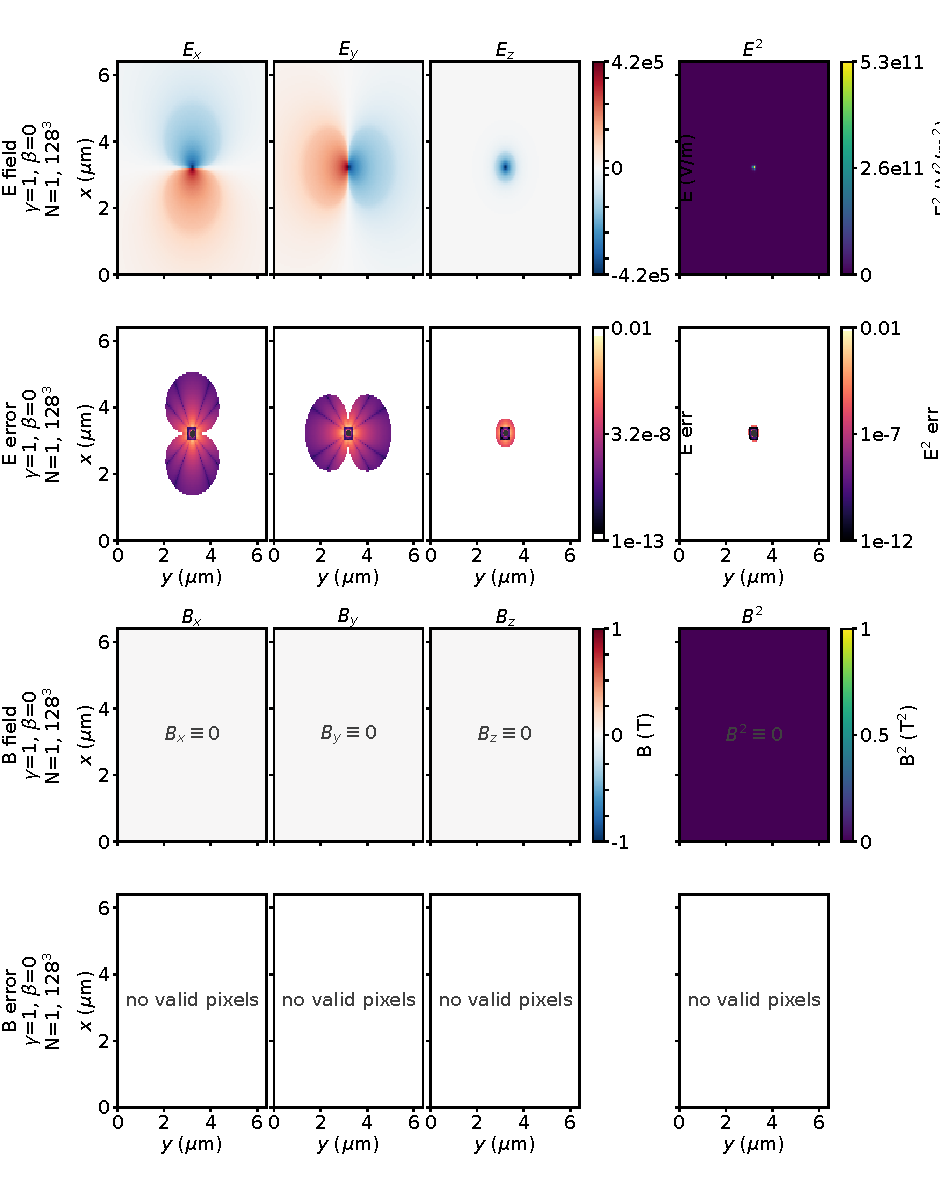
\includegraphics[width=\linewidth]{figs/gp_g1p0.pdf}
\caption{Single-electron field and error on the x-y plane at mid-$z$ for
$\beta=0$ ($\gamma=1.0$) on the $128^3$ grid, cell $5\times10^{-8}$\,m.
The bunch moves along $+y$: $y$ is horizontal and increases to the right,
$x$ is vertical. The $E$ block and the $B$ block each put $E_x,E_y,E_z$ (or $B_x,B_y,B_z$)
on one shared colour scale with its own bar and $E^2$ (or $B^2$) on a
separate colour scale with its own bar, so the squared-magnitude scale never
dominates the component scale. Error rows are logarithmic, carry the
$10^{-3}$ contour, and are masked below $10^{-3}$ of the reference peak; at
$\gamma=1.0$ the $B$ error bars are omitted because no pixel exceeds the
mask threshold; the worst component error is $3.474\times10^{-3}$.}
\label{fig:gp1}
\end{figure}

\begin{figure}[H]
\centering
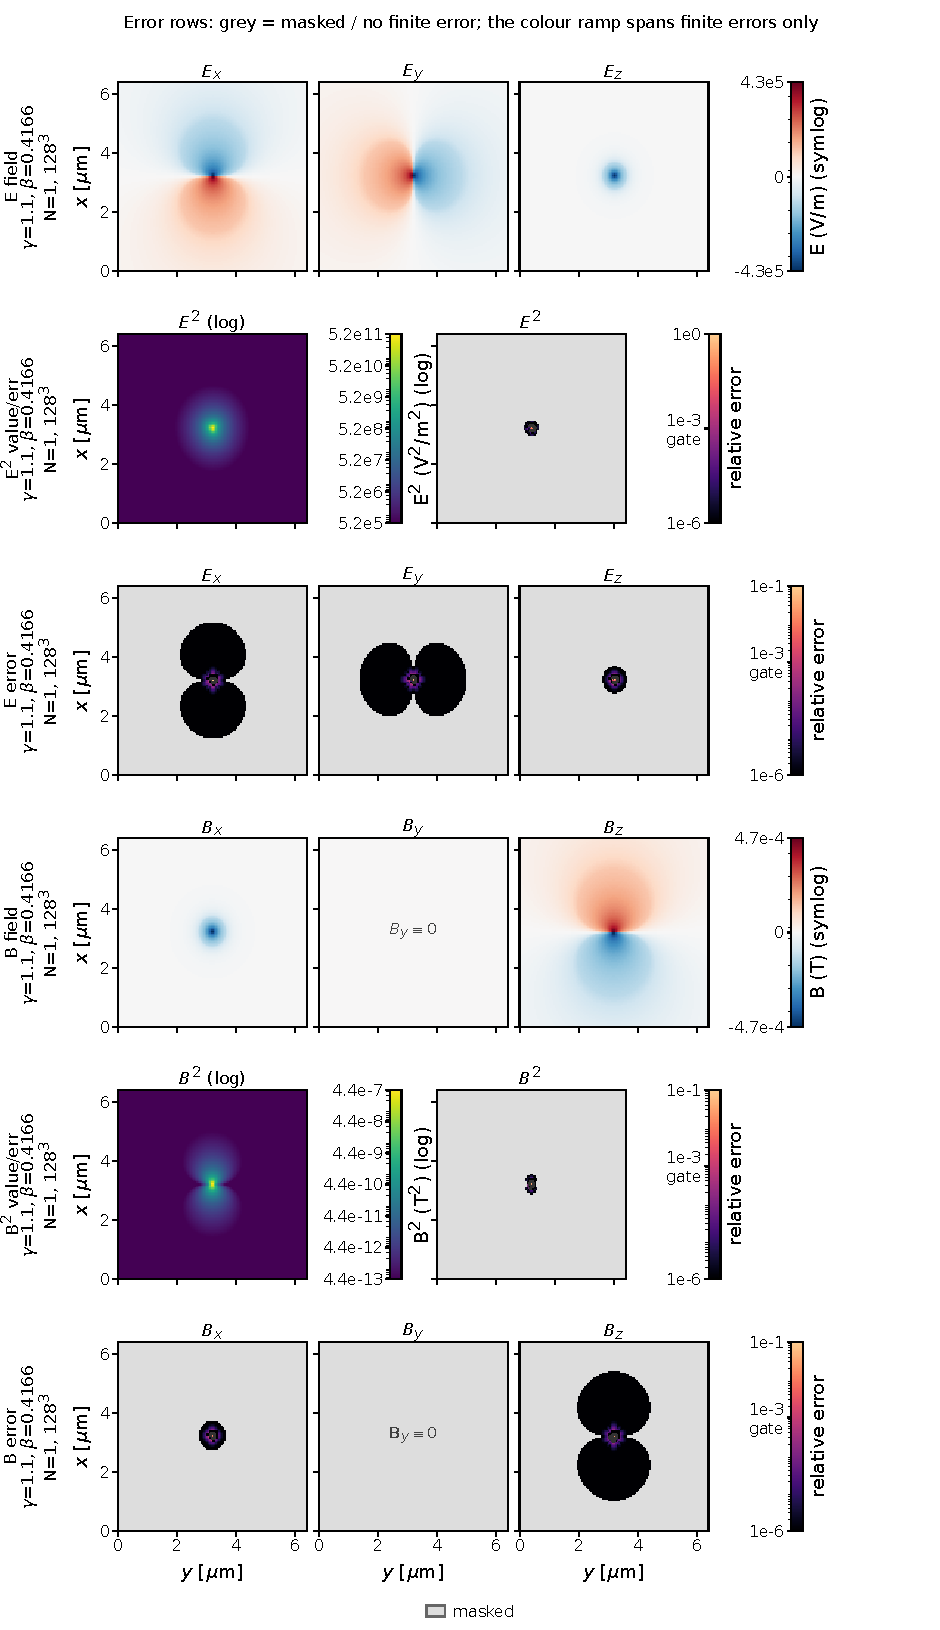
\includegraphics[width=\linewidth]{figs/gp_g1p1.pdf}
\caption{Single-electron field and error on the x-y plane at mid-$z$ for
$\beta=0.4166$ ($\gamma=1.1$) on the $128^3$ grid, cell
$5\times10^{-8}$\,m, with the same field, colour-bar and error conventions
as Fig.~\ref{fig:gp1}. The worst component error is
$3.669\times10^{-3}$.}
\label{fig:gp1p1}
\end{figure}

\begin{figure}[H]
\centering
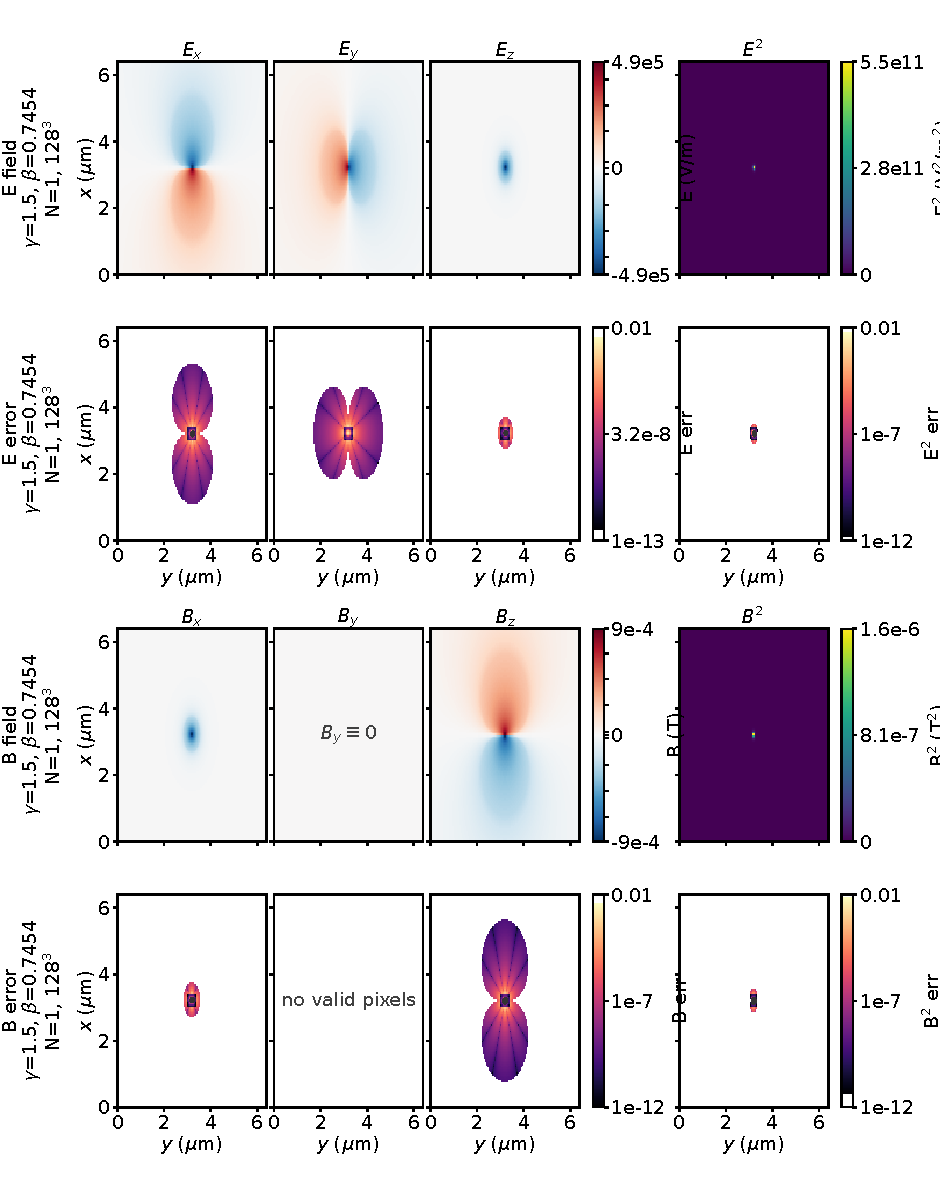
\includegraphics[width=\linewidth]{figs/gp_g1p5.pdf}
\caption{Single-electron field and error on the x-y plane at mid-$z$ for
$\beta=0.7454$ ($\gamma=1.5$) on the $128^3$ grid, cell
$5\times10^{-8}$\,m, with the same field, colour-bar and error conventions
as Fig.~\ref{fig:gp1}. The worst component error is
$3.719\times10^{-3}$.}
\label{fig:gp1p5}
\end{figure}

\begin{figure}[H]
\centering
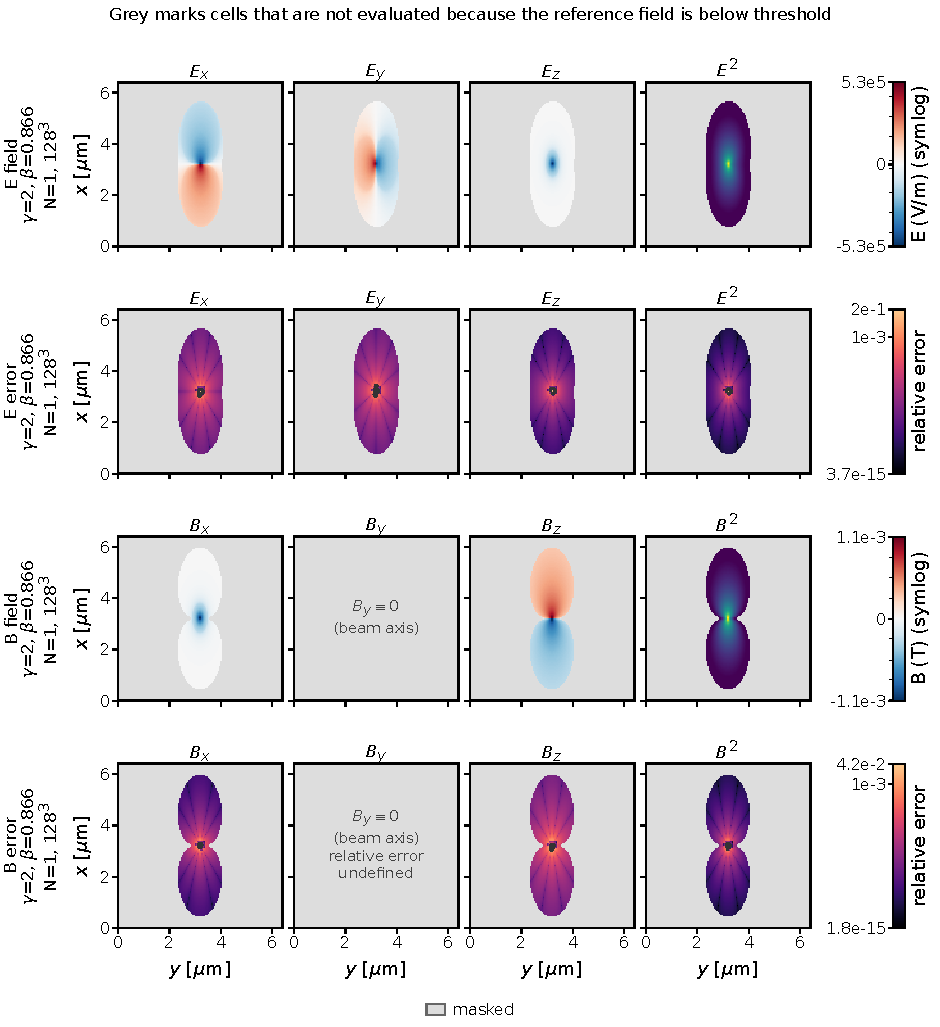
\includegraphics[width=\linewidth]{figs/gp_g2p0.pdf}
\caption{Single-electron field and error on the x-y plane at mid-$z$ for
$\beta=0.8660$ ($\gamma=2.0$) on the $128^3$ grid, cell
$5\times10^{-8}$\,m, with the same field, colour-bar and error conventions
as Fig.~\ref{fig:gp1}. The worst component error is $5.098\times10^{-3}$.}
\label{fig:gp2}
\end{figure}

\begin{figure}[H]
\centering
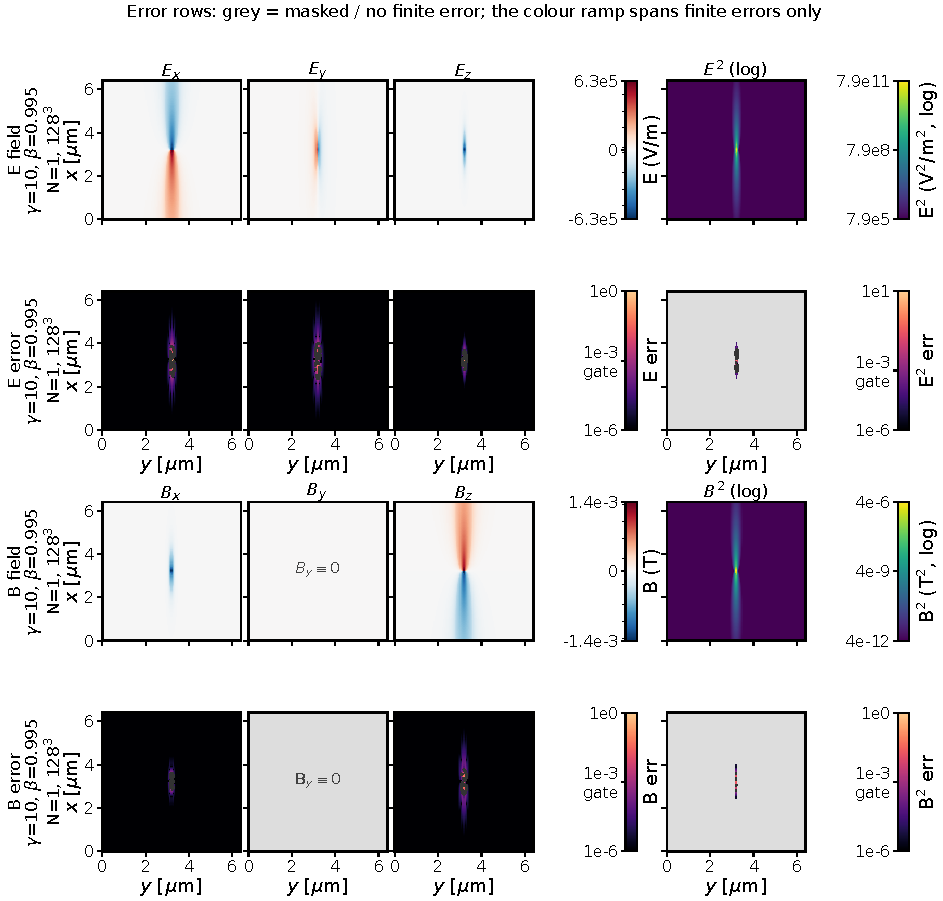
\includegraphics[width=\linewidth]{figs/gp_g10.pdf}
\caption{Single-electron field and error on the x-y plane at mid-$z$ for
$\beta=0.9950$ ($\gamma=10$) on the $128^3$ grid, cell
$5\times10^{-8}$\,m, with the same field, colour-bar and error conventions
as Fig.~\ref{fig:gp1}. The worst component error is
$1.197\times10^{-1}$.}
\label{fig:gp10}
\end{figure}

\begin{figure}[H]
\centering
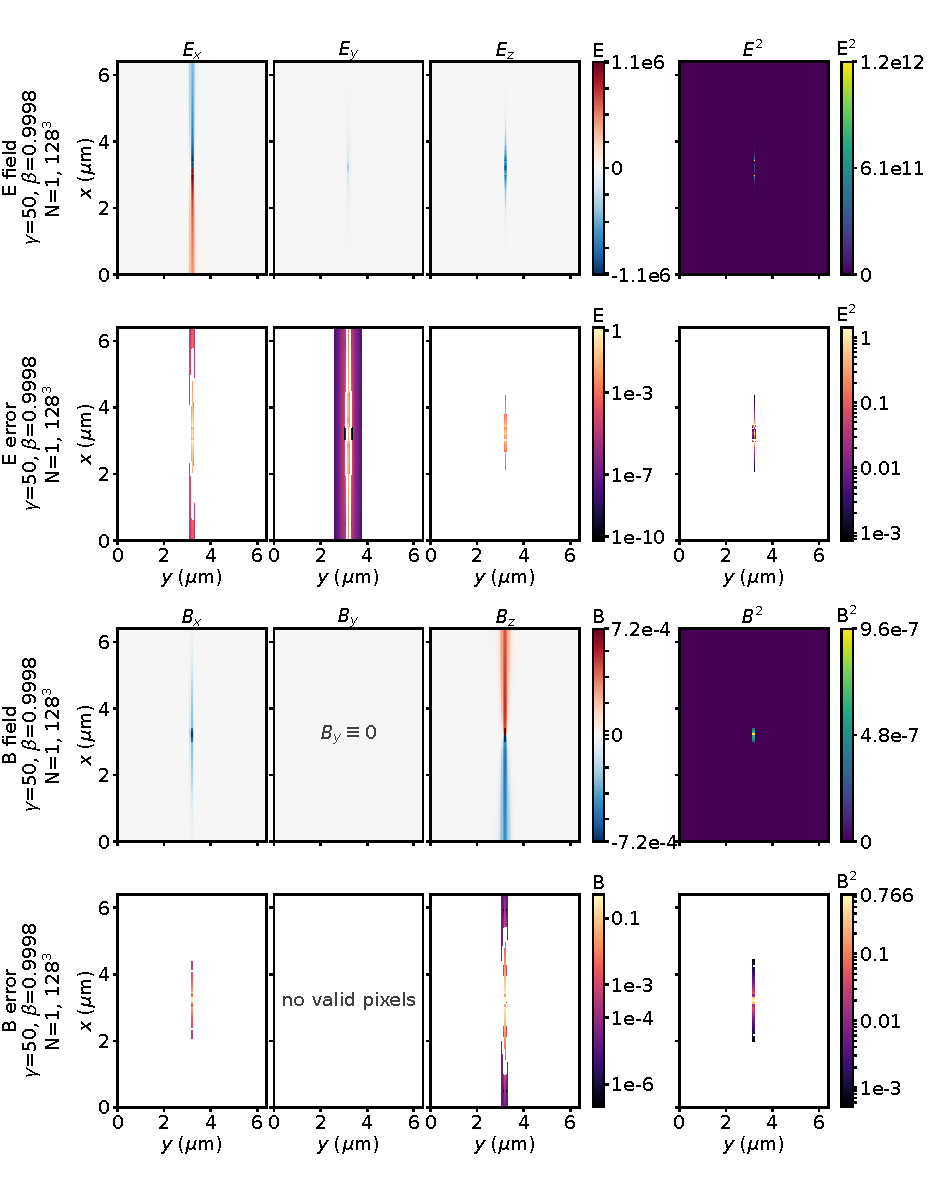
\includegraphics[width=\linewidth]{figs/gp_g50.pdf}
\caption{Single-electron field and error on the x-y plane at mid-$z$ for
$\beta=0.99980$ ($\gamma=50$) on the $128^3$ grid, cell
$5\times10^{-8}$\,m, with the same field, colour-bar and error conventions
as Fig.~\ref{fig:gp1}. The worst component error is $1.426$.}
\label{fig:gp50}
\end{figure}

\begin{figure}[H]
\centering
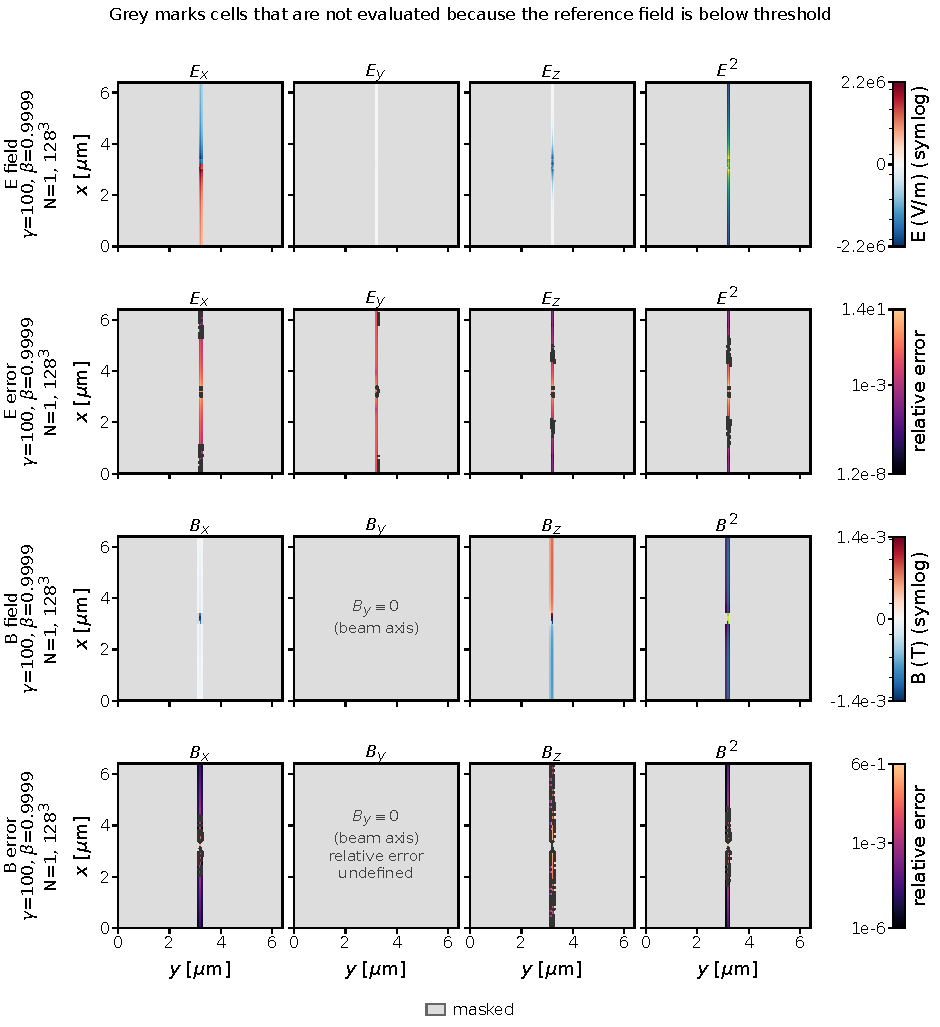
\includegraphics[width=\linewidth]{figs/gp_g100.pdf}
\caption{Single-electron field and error on the x-y plane at mid-$z$ for
$\beta=0.99995$ ($\gamma=100$) on the $128^3$ grid, cell
$5\times10^{-8}$\,m, with the same field, colour-bar and error conventions
as Fig.~\ref{fig:gp1}. The worst component error is $3.213$.}
\label{fig:gp100}
\end{figure}

\section*{Padding and R2C/C2R details}
\label{app:padding}

With $\mathrm{pad}=1$ the cyclic convolution wraps and a
$9.275\times10^{-3}$ periodic-image artefact appears for a single stationary
particle in a $20^3$ box. For a single stationary particle the
$\mathrm{pad}=2$ result agrees with the direct non-cyclic sum to
$3.811\times10^{-16}$ and the $\mathrm{pad}=3$ result to
$1.905\times10^{-16}$; at $\mathrm{pad}\ge2$ the error is at machine
precision ($\le 10^{-15}$). The artefact grows for beamed sources: at
$\mathrm{pad}=1$ the $100$-source $\gamma=10$ cloud shows a
$7.5\times10^{-1}$ worst-component error.

For the R2C/C2R half-spectra the DC bin and the seven self-conjugate even
Nyquist corners must be exactly real; the intermediate Nyquist planes are
Hermitian-paired, not real. The R2C/C2R path matches the C2C path to
$1.665\times10^{-16}$ over all six components.

The $\gamma$-landscape runs of Section~\ref{sec:gamma-landscape} use
padding $1$; the $d=48$ rows carry a small periodic-wraparound floor of
order $10^{-4}$ to $10^{-3}$, so the $d=48$ values are not padding-clean.
